% Editable LaTeX transcription of the provided exam paper.
\documentclass[12pt]{article}
\usepackage[utf8]{inputenc}
\usepackage[T1]{fontenc}
\usepackage{lmodern}
\usepackage{amsmath,amssymb}
\usepackage{geometry}
\usepackage{enumitem}
\usepackage{graphicx}
\usepackage{parskip}
\usepackage{tikz}
\usetikzlibrary{arrows.meta, positioning, shapes, patterns, calc, angles, quotes}
\usepackage{pgfplots}
\pgfplotsset{compat=1.18}

\geometry{a4paper, margin=1in}

\begin{document}

\begin{center}
	{\Large\textbf{SHREE RUDRAPUR SECONDARY SCHOOL (ENGLISH MEDIUM)}}\\[1ex]
	{\large Class : 9 \quad Third Terminal Examination - 2082 \quad F.M : 75}\\[1ex]
	{\large Time : 3 hrs \quad Sub : C. Math}
\end{center}

\vspace{1em}
\noindent\textbf{All questions are compulsory.}

\begin{enumerate}[wide, label=\textbf{\arabic*.}]
	\item Study the given Venn-diagram and answer the following questions.
	\begin{center}
		% Placeholder for the Venn diagram image; replace with actual image if available.
		\fbox{\parbox[c][5cm][c]{0.6\textwidth}{\centering Venn diagram placeholder}}
	\end{center}
	\begin{enumerate}[label=\textbf{\alph*.}, leftmargin=2em]
		\item What type of sets are $A$, $B$ and $C$? (1)
		\item What is the cardinal number of universal set $U$? (1)
		\item Using a Venn-diagram, show that $n(A\cup B)=n(A)+n(B)-n(A\cap B)$. (3)
		\item What is the relation of $n(U)$, $n(A)$ and $n(\overline{A})$? (1)
	\end{enumerate}

	\item If $U=\{1,2,3,4,\dots,9\}$, $A=\{1,2,4,8\}$, $B=\{1,2,3,6\}$ and $C=\{1,3,9\}$
	\begin{enumerate}[label=\textbf{\alph*.}, leftmargin=2em]
		\item Write down the common member of $A$ and $B$. (1)
		\item Find $n(A\cap B\cap C)$. (2)
		\item Prove that $\overline{A\cup B}=\overline{A}\cap\overline{B}$. (3)
	\end{enumerate}

	\item The marked price of a mobile set is Rs. 40,000. The mobile set is sold allowing 10\% discount and
	levying 13\% Value Added Tax.
	\begin{enumerate}[label=\textbf{\alph*.}, leftmargin=2em]
		\item What is the formula to find discount percent when the marked price and SP after discount are given? (1)
		\item Find the discount amount and SP after discount. (2)
		\item Find the VAT amount and SP with VAT. (2)
	\end{enumerate}

	\item A retailer bought an article for Rs. 27,500 without VAT. He fixed the marked price to be Rs. 35,000 and sold
	it at 10\% discount and adding 13\% VAT.
	\begin{enumerate}[label=\textbf{\alph*.}, leftmargin=2em]
		\item What is the discount amount? (1)
		\item Finally, into whose account is the VAT amount deposited? (1)
		\item How much should a customer pay for it? (2)
	\end{enumerate}

	\item A commercial bank sold 25,000 shares in a particular year. If the bank earned a net profit of Rs. 2,40,00,000
	and distributed a certain percent of it as dividend. If a shareholder with 500 shares received Rs. 96,000 as dividend.
	\begin{enumerate}[label=\textbf{\alph*.}, leftmargin=2em]
		\item What is the total dividend amount? (2)
		\item What percent of the profit was distributed as dividend? (2)
		\item How much dividend does a shareholder with 150 shares receive? (1)
	\end{enumerate}

	\item A family uses 325 calls in a month. The charge of the first 175 calls is Rs. 200 and Rs. 1 per extra call is
	charged. If 10\% TSC and 13\% VAT is added in the bill.
	\begin{enumerate}[label=\textbf{\alph*.}, leftmargin=2em]
		\item How much TSC should be paid? (1)
		\item What is the total VAT amount? (1)
		\item What is the total bill amount to be paid? (2)
	\end{enumerate}

	\item
	\begin{enumerate}[label=\textbf{\roman*.}, leftmargin=2em]
		\item Prove that $\dfrac{x+1}{3} + \dfrac{x}{4\times 3} = 1$. (2)
		\item Solve: $\dfrac{x-2}{x+2} = 3$. (1)
		\item Solve: $x-4x=0$. (2)
	\end{enumerate}

	\item A shopkeeper bought a camera for Rs. 800 and fixed its marked price 25\% above the cost price.
	\begin{enumerate}[label=\textbf{\alph*.}, leftmargin=2em]
		\item Find the Marked Price of the camera. (1)
		\item If he sold it by allowing 10\% discount, find the discount amount. (1)
		\item Find the selling price. (1)
		\item Find Profit or loss amount. (1)
	\end{enumerate}

	\item Answer the following questions on the basis of two equations written by a teacher on the board.
	\begin{enumerate}[label=\textbf{\alph*.}, leftmargin=2em]
		\item What types of lines — either straight or curve — are represented by the given linear equations? (1)
		\item Solve the above equations. (2)
		\item From the linear equation satisfying $x=3$ and $y=4$. (1)
	\end{enumerate}

	\item The given sequence is an A.P.: $20,15,10,5,0,-5,\dots$
	\begin{enumerate}[label=\textbf{\alph*.}, leftmargin=2em]
		\item Write the formula to find the general term of an A.P. (1)
		\item Find the 8th term $t_8$ of the sequence. (2)
	\end{enumerate}

	\item Answer the following questions.
	\begin{enumerate}[label=\textbf{\alph*.}, leftmargin=2em]
		\item What type of series is called an arithmetic series? (1)
		\item Find the value of $\displaystyle\sum_{n=1}^{5} n(2+2n+1)$. (2)
		\item If $x-3$, $x$ and $x+3$ are in geometric sequence, find the value of $x$. (2)
	\end{enumerate}

	\item
	\begin{enumerate}[label=\textbf{\alph*.}, leftmargin=2em]
		\item Factorize: $a^{2}-2a+2b-b^{2}$. (3)
		\item Find the H.C.F. of $8x^{3}+y$ and $16x^{4}+4x^{2}y+y^{2}$. (3)
	\end{enumerate}

	\item
	\begin{enumerate}[label=\textbf{\alph*.}, leftmargin=2em]
		\item Find the L.C.M. of $x^{2}-9$, $x^{3}+27$ and $x+9x+81$. (2)
		\item Simplify the following expression: (3)\\
		\[\left(\dfrac{a}{x}\right)^{2}+\dfrac{2}{a+ab+b}\times\left(\dfrac{b}{x}\right)^{2}+\dfrac{2}{b+bc+c}\times\left(\dfrac{c}{x}\right)^{2}+\dfrac{2}{c+ca+a}\]
	\end{enumerate}

	\item
	\begin{enumerate}[label=\textbf{\alph*.}, leftmargin=2em]
		\item Find the value of $\;y-2\;$ when (context missing). (1)
		\item If $a=4$ and $b=5$, find the value of $\dfrac{a^{2}}{a+2ab+b^{2}}$. (1)
		\item If $a+b+c=0$ prove that:
		\[\frac{1}{1+x+x^{2}}\left(\frac{b}{b-c}\right)+\frac{1}{1+x+x^{2}}\left(\frac{c}{c-a}\right)+\frac{1}{1+x+x^{2}}\left(\frac{a}{a-b}\right)=1.\]
	\end{enumerate}

	\item At present, Rita's age is 3 times her daughter's age. Fifteen years ago, the sum of their ages was 34 years.
	\begin{enumerate}[label=\textbf{\alph*.}, leftmargin=2em]
		\item Write the above statements in the form of linear equations. (1)
		\item Find their present ages. (2)
	\end{enumerate}

	\item The total cost of 4 kg of potatoes and 2 kg of onions is Rs. 350. If the cost of 3 kg potatoes is same as
	the cost of 2 kg of onions.
	\begin{enumerate}[label=\textbf{\alph*.}, leftmargin=2em]
		\item Express the above conditions in the form of linear equations. (1)
		\item Find the per kg cost of each item. (2)
		\item If a man buys 15 kg of potatoes and 10 kg of onions how much should he pay for it? (2)
	\end{enumerate}
\end{enumerate}

\clearpage
\section*{Additional Practice: Illustrated Questions}
\begin{enumerate}[wide, label=\textbf{Q\arabic*.}]
	\item (Triangle geometry) In triangle $ABC$ below, $AB=7$, $AC=8$ and $\angle A=60^\circ$. Find the area of $\triangle ABC$.\\
	\begin{center}
		\begin{tikzpicture}[scale=1]
			\coordinate (A) at (0,0);
			\coordinate (B) at (3,0);
			\coordinate (C) at (1.5,2.598); % approx for 60 deg
			\draw (A) -- (B) -- (C) -- cycle;
			\node[below left] at (A) {A};
			\node[below right] at (B) {B};
			\node[above] at (C) {C};
			\draw pic[draw, ->, angle radius=6mm] {angle = B--A--C};
			\node at (0.6,0.25) {$60^\circ$};
		\end{tikzpicture}
	\end{center}

	\item (Function graph) Sketch the graph of $y=x^2-4x+3$ and state its vertex and the x-intercepts.\\
	\begin{center}
		\begin{tikzpicture}
			\begin{axis}[width=8cm,axis lines=middle, xlabel=$x$, ylabel=$y$, xmin=-1, xmax=5, ymin=-1, ymax=6]
				\addplot[domain=-1:5,samples=200,blue,thick] {x^2-4*x+3};
				\addplot[only marks,mark=*,red] coordinates {(1,0) (3,0)};
				\addplot[only marks,mark=*,black] coordinates {(2,-1)};
			\end{axis}
		\end{tikzpicture}
	\end{center}

	\item (Bar chart) The scores of five students are shown. Which student scored the highest?\\
	\begin{center}
		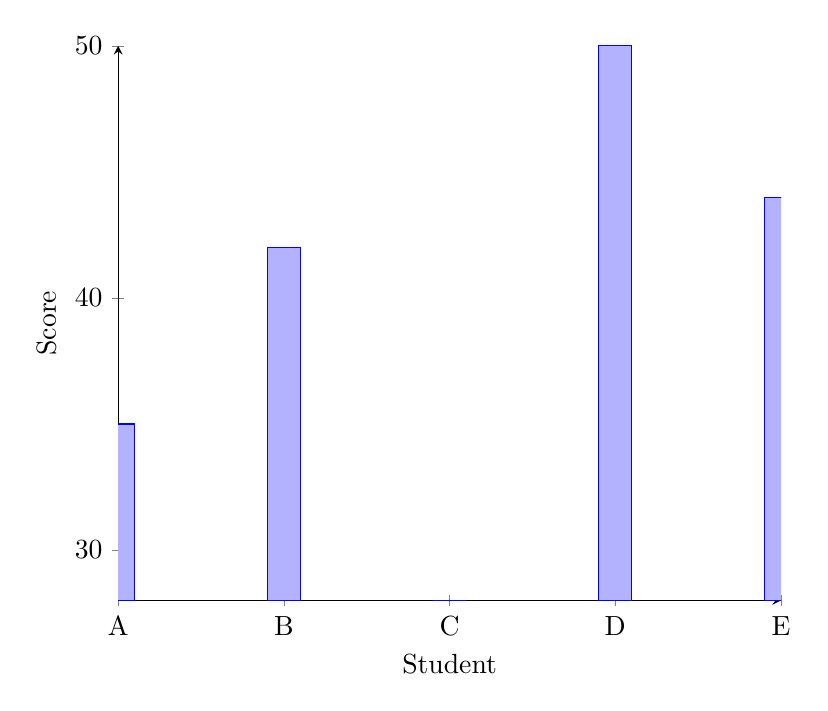
\begin{tikzpicture}
			\begin{axis}[ybar,bar width=12pt,ytick={0,10,20,30,40,50},width=10cm,axis x line=bottom,axis y line=left,xlabel=Student, ylabel=Score,xtick=data,xticklabels={A,B,C,D,E}]
				\addplot coordinates {(1,35) (2,42) (3,28) (4,50) (5,44)};
			\end{axis}
		\end{tikzpicture}
	\end{center}

	\item (Venn diagram) Shade the region corresponding to $A\cap(B\setminus C)$ in the diagram below.\\
	\begin{center}
		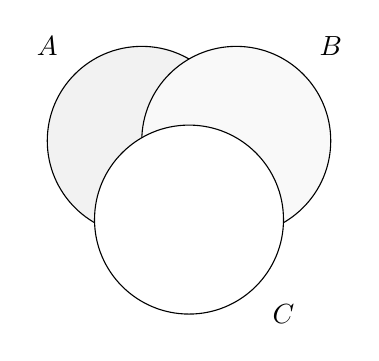
\begin{tikzpicture}
			\draw[fill=gray!10] (0,0) circle (1.2) node at (-1.2,1.2) {$A$};
			\draw[fill=gray!5] (1.2,0) circle (1.2) node at (2.4,1.2) {$B$};
			\draw[fill=white] (0.6,-1) circle (1.2) node at (1.8,-2.2) {$C$};
			% label regions roughly
		\end{tikzpicture}
	\end{center}

	\item (Coordinate geometry) Points $P(1,2)$, $Q(4,6)$ and $R(7,2)$ form a triangle. Find its area.\\
	\begin{center}
		\begin{tikzpicture}[scale=0.6]
			\draw[->] (-1,0) -- (9,0) node[right] {$x$};
			\draw[->] (0,-1) -- (0,8) node[above] {$y$};
			\foreach \x in {1,2,...,8} \draw (\x,0.1) -- (\x,-0.1);
			\foreach \y in {1,2,...,7} \draw (0.1,\y) -- (-0.1,\y);
			\coordinate (P) at (1,2);
			\coordinate (Q) at (4,6);
			\coordinate (R) at (7,2);
			\draw[thick] (P) -- (Q) -- (R) -- cycle;
			\fill (P) circle (2pt) node[below left] {P(1,2)};
			\fill (Q) circle (2pt) node[above] {Q(4,6)};
			\fill (R) circle (2pt) node[below right] {R(7,2)};
		\end{tikzpicture}
	\end{center}

	\item (Pie-like sectors) A survey shows categories with proportions 30\%, 25\%, 20\%, 15\%, 10\%. Draw a pie-like sector diagram and label the largest sector.\\
	\begin{center}
		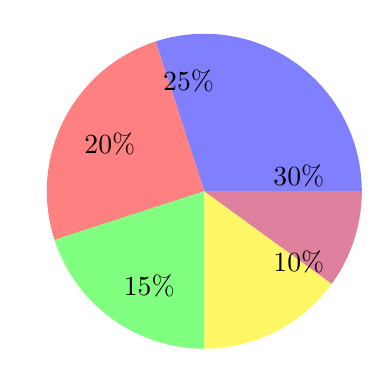
\begin{tikzpicture}[scale=1]
			\def\start{0}
			\def\a{360*0.30}
			\def\b{360*0.25}
			\def\c{360*0.20}
			\def\d{360*0.15}
			\def\e{360*0.10}
			\fill[blue!50] (0,0) -- (\start:2) arc (\start:\start+\a:2) -- cycle;
			\fill[red!50] (0,0) -- (\start+\a:2) arc (\start+\a:\start+\a+\b:2) -- cycle;
			\fill[green!50] (0,0) -- (\start+\a+\b:2) arc (\start+\a+\b:\start+\a+\b+\c:2) -- cycle;
			\fill[yellow!60] (0,0) -- (\start+\a+\b+\c:2) arc (\start+\a+\b+\c:\start+\a+\b+\c+\d:2) -- cycle;
			\fill[purple!50] (0,0) -- (\start+\a+\b+\c+\d:2) arc (\start+\a+\b+\c+\d:360:2) -- cycle;
			\node at (1.2,0.2) {30\%};
			\node at (-0.2,1.4) {25\%};
			\node at (-1.2,0.6) {20\%};
			\node at (-0.7,-1.2) {15\%};
			\node at (1.2,-0.9) {10\%};
		\end{tikzpicture}
	\end{center}

	\item (Network graph) In the graph below, edges have weights. Find the shortest path from $S$ to $T$.\\
	\begin{center}
		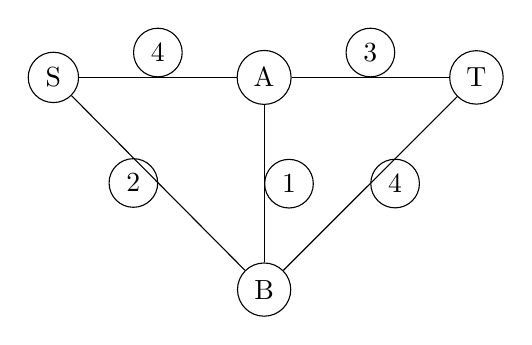
\begin{tikzpicture}[node distance=2cm, every node/.style={circle,draw}]
			\node (S) {S};
			\node (A) [right=of S] {A};
			\node (B) [below=of A] {B};
			\node (T) [right=of A] {T};
			\draw (S) -- node[above] {4} (A) -- node[above] {3} (T);
			\draw (S) -- node[left] {2} (B) -- node[right] {4} (T);
			\draw (A) -- node[right] {1} (B);
		\end{tikzpicture}
	\end{center}

	\item (Histogram) The frequency of values is shown; estimate the mean approximately from the chart.\\
	\begin{center}
		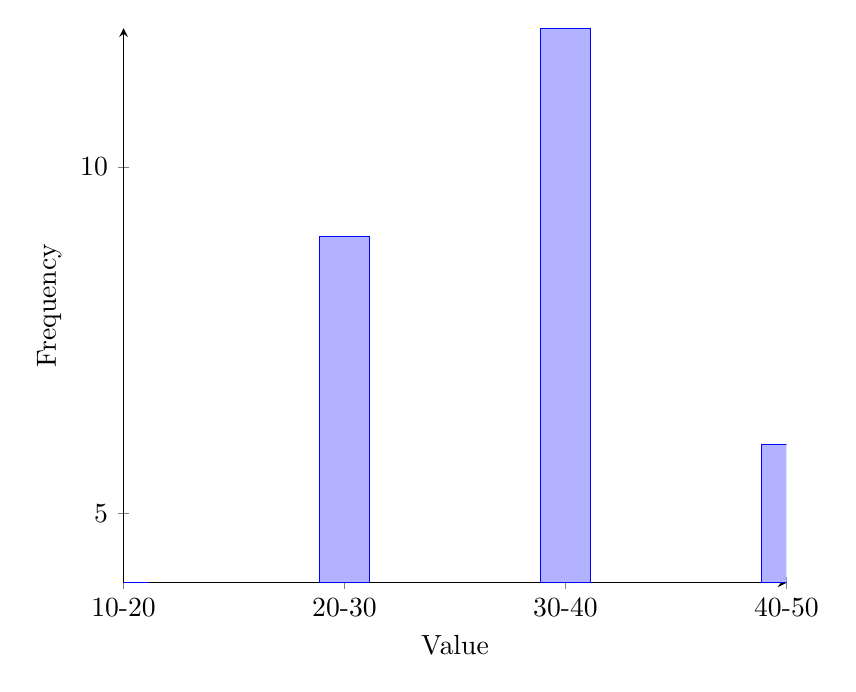
\begin{tikzpicture}
			\begin{axis}[ybar,bar width=18pt,ytick align=outside,ytick={0,5,10,15},width=10cm,axis x line=bottom,axis y line=left,xlabel=Value, ylabel=Frequency,xtick=data,xticklabels={10-20,20-30,30-40,40-50}]
				\addplot coordinates {(1,4) (2,9) (3,12) (4,6)};
			\end{axis}
		\end{tikzpicture}
	\end{center}

	\item (Trigonometry on unit circle) Mark an angle $\theta=50^\circ$ and show $\sin\theta$ and $\cos\theta$ on the diagram.\\
	\begin{center}
		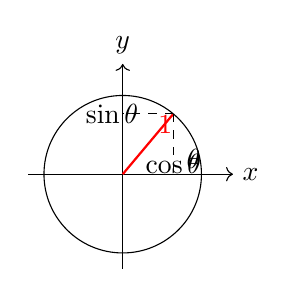
\begin{tikzpicture}[scale=1]
			\draw (0,0) circle (1);
			\draw[->] (-1.2,0) -- (1.4,0) node[right] {$x$};
			\draw[->] (0,-1.2) -- (0,1.4) node[above] {$y$};
			\coordinate (P) at ({cos(50)},{sin(50)});
			\draw[thick,red] (0,0) -- (P) node[midway,above right] {$1$};
			\draw[dashed] (P) -- ({cos(50)},0) node[midway,below] {$\cos\theta$};
			\draw[dashed] (P) -- (0,{sin(50)}) node[midway,left] {$\sin\theta$};
			\node at (0.9,0.2) {$\theta$};
		\end{tikzpicture}
	\end{center}

	\item (Flowchart/complex diagram) Study the flow and answer which decision leads to output Z.\\
	\begin{center}
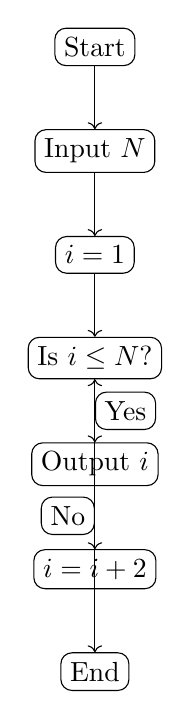
\begin{tikzpicture}[node distance=8mm, every node/.style={rectangle,draw,rounded corners,align=center}]
  \node (start) {Start};
  \node (inp) [below=of start] {Input $N$};
  \node (init) [below=of inp] {$i=1$};
  \node (dec) [below=of init] {Is $i\le N$?};
  \node (out) [below=of dec] {Output $i$};
  \node (inc) [below=of out] {$i=i+2$};
  \node (end) [below=of inc] {End};
  \draw[->] (start) -- (inp);
  \draw[->] (inp) -- (init);
  \draw[->] (init) -- (dec);
  \draw[->] (dec) -- node[right]{Yes} (out);
  \draw[->] (out) -- (inc);
  \draw[->] (inc) -- (dec);
  \draw[->] (dec) -- node[left]{No} (end);
\end{tikzpicture}
\end{center}
\end{enumerate}

\vfill
\begin{center}\textit{The End}\end{center}

\end{document}

